\documentclass[APA,LATO1COL]{WileyNJD-v2}

\articletype{Article Type}%

\usepackage{listings}
\usepackage{hyperref}
\usepackage{graphicx}
\graphicspath{{images/}}


\received{26 April 2016}
\revised{6 June 2016}
\accepted{6 June 2016}

\raggedbottom

\begin{document}

\title{Creating optimal conditions for reproducible data analysis in R with `fertile'\protect\thanks{The authors gratefully acknowledge contributions from Hadley Wickham, Jenny Bryan, Greg Wilson, Edgar Ruiz, and other members of the tidyverse team.}}

\author[1]{Audrey Bertin}

\author[2]{Benjamin S. Baumer}


\authormark{Bertin and Baumer, 2020}


\address[1]{\orgdiv{Program in Statistical and Data Sciences}, \orgname{Smith College}, \orgaddress{\city{Northampton}, \state{MA}}}

\address[2]{\orgdiv{Assistant Professor of Statistical and Data Sciences}, \orgname{Smith College}, \orgaddress{\city{Northampton}, \state{MA}}}


\corres{Audrey Bertin, Program in Statistical and Data Sciences, Smith College, Northampton, MA, 01063. \email{abertin@smith.edu}}


\abstract[Summary]{The advancement of scientific knowledge increasingly depends on ensuring that data-driven research is reproducible: that two people with the same data obtain the same results. However, while the necessity of reproducibility is clear, there are significant behavioral and technical challenges that impede its widespread implementation, and no clear consensus on standards of what constitutes reproducibility in published research. We focus on a series of common mistakes programmers make while conducting data science projects in R, primarily through the RStudio integrated development environment. \textbf{fertile} is an R package that operates in two modes: proactively (to prevent reproducibility mistakes from happening in the first place), and retroactively (analyzing code that is already written for potential problems). Furthermore, \textbf{fertile} is designed to educate the user about why the mistakes are problematic, and how to fix them.}

\keywords{reproducibility, statistical software, workflow, collaboration}


\maketitle

\section{Introduction}\label{sec1}

As research is becoming increasingly data-driven, and because knowledge can be shared worldwide so rapidly, reproducibility is critical to the advancement of scientific knowledge. 
Data-based research cannot be fully reproducible unless the requisite code and data files
produce identical results when run by another analyst. When researchers provide the code and data used for their work in a well-organized and reproducible format, readers are more easily able to determine the veracity of any findings by following the steps from raw data to conclusions.

The creators of reproducible research can more easily receive more specific feedback (including bug fixes) on their work. Moreover, others interested in the research topic can use the code to apply the methods and ideas used in one project to their own work with minimal effort.

However, while the necessity of reproducibility is clear, there are significant behavioral and technical challenges that impede its widespread implementation, and no clear consensus on standards of what constitutes reproducibility in published research (\cite{peng2009bio}). Not only are the components of reproducible research up for discussion (e.g., need the software be open source?), but the corresponding recommendations for ensuring reproducibility also vary (e.g., should raw and processed data files be in separate directories?).

Much of the discussion around reproducibility is also generalized, written to be applicable to users working with a variety of statistical software programs. Since all statistical software programs operate differently, generalized recommendations on reproducibility are often shallow and unspecific. While they provide useful guidelines, they can often be difficult to implement, particularly to new analysts who are unsure how to apply such recommendations within the software programs they are using. Thus, reproducibility recommendations tailored to specific software programs are more likely to be adopted.

In this paper, we focus on reproducibility in the R programming language with a concentration on projects that use the RStudio integrated development environment. R is an ideal candidate for reproducibility recommendations due to the language's popularity for statistical analyses and the ease with which analysts can download and begin using the software.

A small body of papers and R packages focusing on reproducibility in the R community have been published. Much of this work is narrowly tailored, with each package effectively addressising a small component of reproducibility: file structure, modularization of code, version control, etc. Many existing reproducibility packages, due to their focused nature, succeed at their area of focus, but at a cost. They are often difficult to learn and operate, providing a barrier to entry for less-experienced data analysts.

There appear to be no existing tools that cater to analysts looking for an easy-to-learn, easy-to-implement, fast, way to obtain a broad overview of their projects' reproducibility. To address this, we present an R package called \textbf{fertile}, a low barrier-to-entry package which focuses on a series of common mistakes programmers make while conducting data science research in R.



\section{Literature Review}\label{sec2}


Reproducibility is critically important to the advancement of knowledge in all fields of scientific research. Researchers are acknowledging this; publications and discussions focusing on reproducibility seem to have increased in frequency over the last several years. (\cite{sep-scientific-reproducibility}, \cite{plos-biology}, \cite{bioessays-gosselin}, \cite{eisner-reproducibility}, \cite{engineering-reproducibility})

Much of the available literature is focused on the methods for achieving reproducibility in specific disciplines, though much of this information is generalizable to all areas of scientific research. There is also work focusing specifically on reproducibility within the R community. Some of this work is in the form of academic papers, while other literature comes from blog posts, websites, and R packages, some of which are compiled by notable R-focused developers and researchers. In this section, we will discuss the reproducibility recommendations from both the formal and informal publications, which together influence the development of \textbf{fertile}.


\subsection{Previous Work}

\cite{Goodman341ps12} argues that the language and conceptual framework of research reproducibility varies across the sciences. There are no clear standards agreed upon across fields.

\cite{kitzes2017practice} presents a collection of case studies on reproducibility practices from across the data-intensive sciences, illustrating a variety of recommendations and techniques for achieving reproducibility. Although the book does not come to a consensus on the exact standards of reproducibility that should be followed, several common trends and principles emerge from the case studies:

\begin{itemize}
\item[1] Use clear separation, labeling, and documentation.
\item[2] Automate processes when possible.
\item[3] Design the data analysis workflow as a sequence of small steps glued together, with
outputs from one step serving as inputs into the next. This is a common suggestion within the computing community, originating as part of the Unix philosophy (Gancarz (2002)).
\end{itemize}


\cite{cooper2017guide} focuses on data analysis in R and identifies similar important reproducibility components, while reiterating the need for clearly labeled, well-documented, and well-separated files. In addition, they recommend publishing a list of dependencies and using version control.

Broman reiterates the need for clear naming and file separation while sharing several additional suggestions: keep the project contained in one directory, use relative paths, and include a \textit{README} (\cite{broman}).

The reproducibility recommendations from R OpenSci, a non-profit initiative founded in 2011 to make scientific data retrieval reproducible, share similar principles to those discussed previously. They focus on a need for a well-developed file system, with no extraneous files and clear labeling. They also reiterate the need to note dependencies and use automation when possible, while making clear a suggestion not present in the previously-discussed literature: the need to use seeds, which allow for the saving and restoring of the random number generator state, when running code involving randomness (\cite{r-opensci}).

When considered in combination, these sources provide a well-rounded picture of the components important to research reproducibility. Using this literature as a guideline, we identify several key features of reproducible work to focus on. These recommendations are opinionated—due to the lack of agreement on which components of reproducibility are most important, we select those that are mentioned most often, as well as some that are mentioned less but that we view as important.

\vskip 0.5in


\begin{itemize}
\item[1] A well-designed file structure:
  \begin{itemize}
  \item Separate folders for different file types.
  \item No extraneous files.
  \item Minimal clutter.
  \end{itemize}
\item[2] Good documentation:
  \begin{itemize}
  \item Files are clearly named, preferably in a way where the order in which they should be run is clear.
  \item A README is present.
  \item Dependencies are noted.
  \end{itemize}
\item[3] Reproducible file paths:
  \begin{itemize}
  \item No absolute paths, or paths leading to locations outside of a project’s directory, are used in code. Only portable (relative) paths.
  \end{itemize}
\item[4] Randomness is accounted for:
  \begin{itemize}
  \item If randomness is used in code, a seed must also be set.
  \end{itemize}
\item[5] Code conforms to tidyverse style:
  \begin{itemize}
  \item Although not discussed in any of the literature mentioned previously, we also believe \textbf{tidyverse} integration to be very important. Code conformation to \textbf{tidyverse} style helps ensure that analyses meeting \textbf{fertile}'s recommendations will be able to integrate seamlessly with packages from the \textbf{tidyverse}, an ever-expanding collection of packages designed to operate together with one another.
  \end{itemize}
\end{itemize}

  
Much of the available literature focuses on file structure, organization, and naming, and \textbf{fertile}'s features are consistent with this. The ideal file structure is not agreed upon by academics, though there are some recommendations focused on R that are available. \cite{marwick2018packaging} provides the framework for file structure that \textbf{fertile} is based on: a structure similar to that of an R package (\cite{hadley-packages}, \cite{coreteam-extensions}), with an \textit{R} folder, as well as \textit{data}, \textit{data-raw}, \textit{inst} and \textit{vignettes}.

\subsection{R Packages}

A small selection of R packages work to address the issue of research reproducibility, although not all of them are available on CRAN.

\textbf{rrtools} (\cite{R-rrtools}) addresses some of the issues discussed in \cite{marwick2018packaging} by creating a basic R package structure for a data analysis project and implementing a basic \textit{testthat::check} functionality. The \textbf{orderly} (\cite{R-orderly}) package also focuses on file structure, requiring the user to declare a desired project structure (typically a step-by-step structure, where outputs from one step are inputs into the next) at the beginning and then creating the files necessary to achieve that structure. \textbf{workflowr}'s (\cite{R-workflowr}) functionality is based around version control and making code easily available online. It works to generate a website containing time-stamped, versioned, and documented results. \textbf{checkers} (\cite{R-checkers}) allows you to create custom checks that examine different aspects of reproducibility. \textbf{packrat} (\cite{R-packrat}) is focused on dependencies, creating a packaged folder containing a project as well as all of its dependencies, so that projects dependent on lesser-used packages can be easily shared across computers. \textbf{drake} (\cite{R-drake}) works to analyze workflows, skip steps where results are up to date, and provide evidence that results match the underlying code and data. Lastly, the \textbf{reproducible} (\cite{R-reproducible}) package focuses on the concept of caching: saving information so that projects can be run faster each time they are re-completed from the start.

Many of these packages focus on one specific area of reproducibility, and while they each succeed well at their intended goal, they are not necessarily the most practical option for users trying to address a wide variety of factors influencing reproducibility at once.

Additionally, with the focused nature of these packages comes added complexity. The functions in these packages are often quite complex to use, and many steps must be completed to achieve the required reproducibility goal. This cumbersome nature means that most reproducibility packages currently available are not easily accessible to users near the beginning of their R journey, nor particularly useful to those looking for quick and easy reproducibility checks.

\section{Methods}\label{sec3}

\textbf{fertile} addresses these gaps by providing a simple, easy-to-learn reproducibility package that, rather than focusing intensely on a specific area, provides some information about a wide variety of aspects influencing reproducibility. The package also provides flexibility, offering benefits to users at any stage in the data analysis workflow, unlike some other available packages which can only be used before the creation of a new project or after it is finished.

\textbf{fertile} is designed to be used on data analyses organized as R Projects (i.e. directories containing an \textit{.Rproj} file). Once an R Project is created, \textbf{fertile} provides benefits throughout the data analysis process, both during development as well as after the fact. \textbf{fertile} achieves this by operating in two modes: proactively (to prevent reproducibility mistakes from happening in the first place), and retroactively (analyzing code that has already been written for potential problems).

\subsection{Proactive Use}

Proactively, the package identifies potential mistakes as they are made by the user and outputs an informative message as well as a recommended solution. For example, \textbf{fertile} catches when a user passes a potentially problematic file path--such as an absolute path, or a path that points to a location outside of the project directory--to a variety of common input/output functions operating on many different file types.

\vskip 0.25in

\centerline{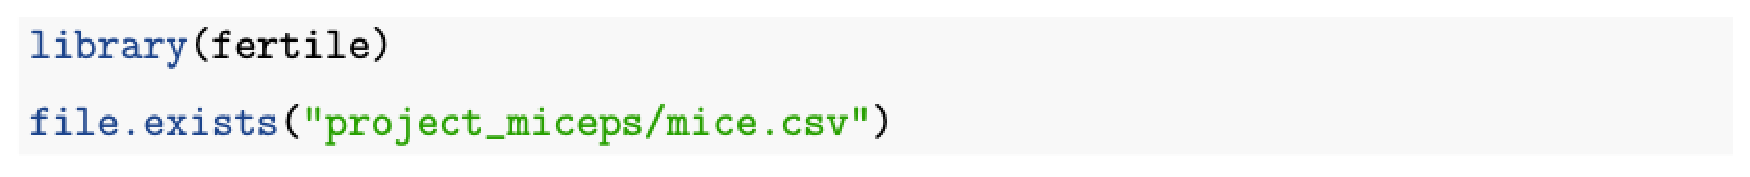
\includegraphics[height=3pc,width=180mm]{fig-1}}
\centerline{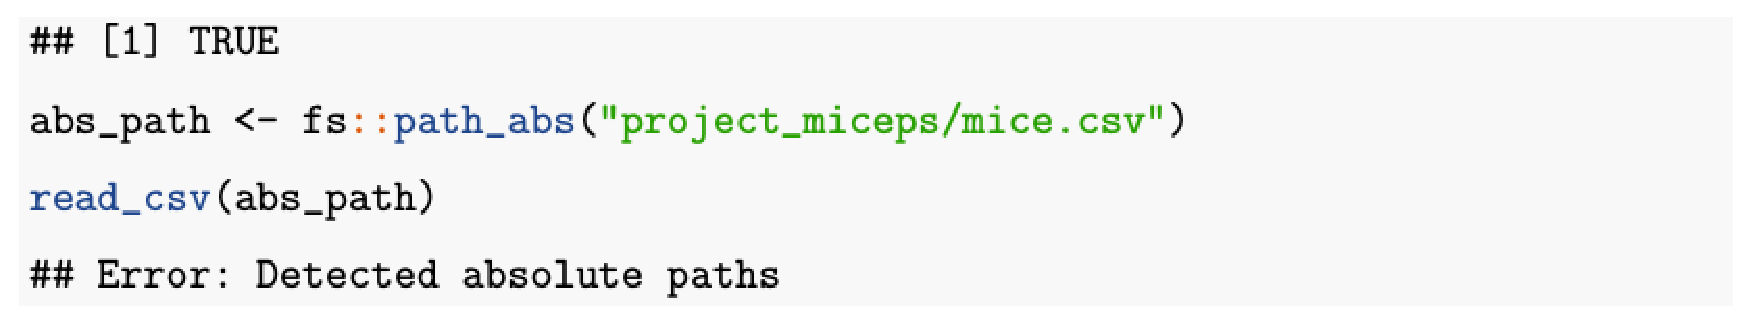
\includegraphics[height=6pc,width=180mm]{fig-2}}

\vskip 0.25in


\textbf{fertile} is even more aggressive with functions (like \textit{setwd()}) that are almost certain to break reproducibility, causing them to throw errors that prevent their execution and providing recommendations for better alternatives.

\vskip 0.25in

\centerline{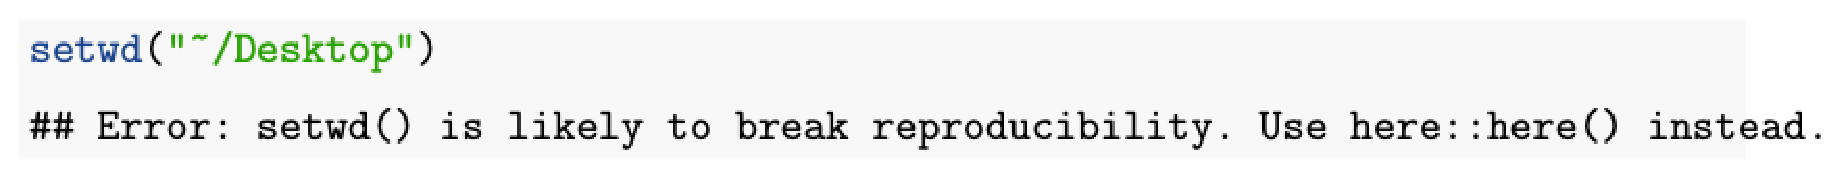
\includegraphics[height=3pc,width=180mm]{fig-3}}

\vskip 0.25in

These proactive warning features are activated immediately after attaching the \textbf{fertile} package and require no additional effort by the user.

\subsection{Retroactive Use}

Retroactively, \textbf{fertile} analyzes potential obstacles to reproducibility in an RStudio Project (i.e., a directory that contains an \textit{.Rproj} file). The package considers several different aspects of the project which may influence reproducibility, including the directory structure, file paths, and whether randomness is used thoughtfully.

The end products of these analyses are reproducibility reports summarizing a project's adherence to reproducibility standards and recommending remedies for where the project falls short. For example, \textbf{fertile} might identify the use of randomness in code and recommend setting a seed if one is not present.

Users can access the majority of \textbf{fertile}'s retroactive features through two primary functions, \textit{proj\_check()} and \textit{proj\_analyze()}.

The \textit{proj\_check()} function runs fifteen different reproducibility tests, noting which ones passed, which ones failed, the reason for failure, a recommended solution, and a guide to where to look for help. These tests include: looking for a clear build chain, checking to make sure the root level of the project is clear of clutter, confirming that there are no files present that are not being directly used by or created by the code, and looking for uses of randomness that to not have a call to \textit{set.seed()} present. A full list is provided below:

\vskip 0.25in

\centerline{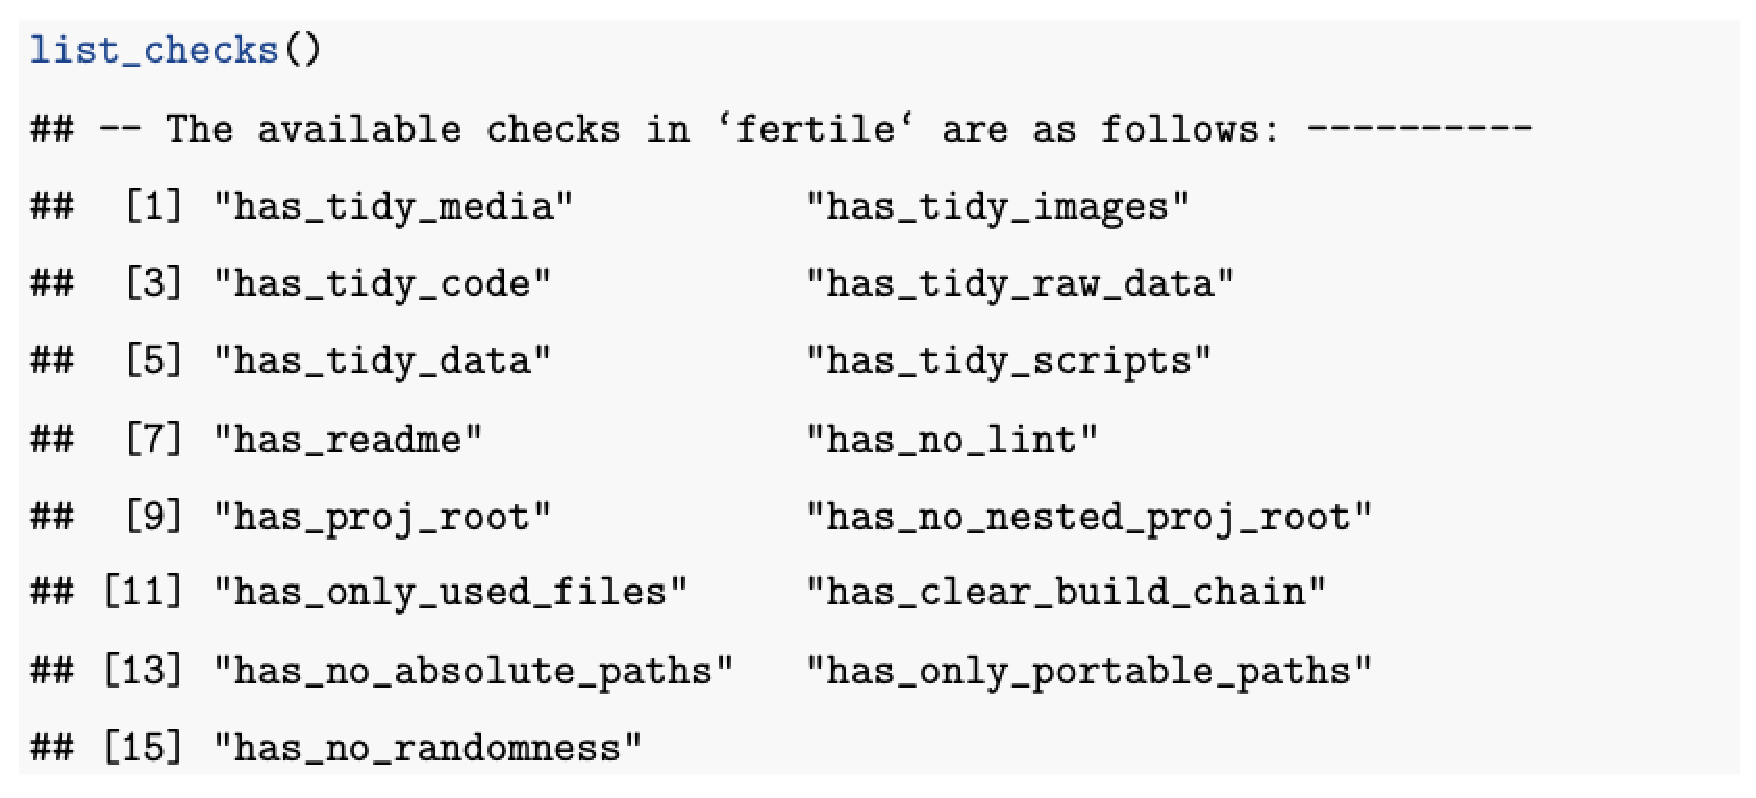
\includegraphics[height=16pc,width=180mm]{fig-4}}

\vskip 0.25in

Subsets of the fifteen tests can be invoked using the tidyselect helper functions in combination with the more limited \textit{proj\_check\_some()} function.

\vskip 0.25in

\centerline{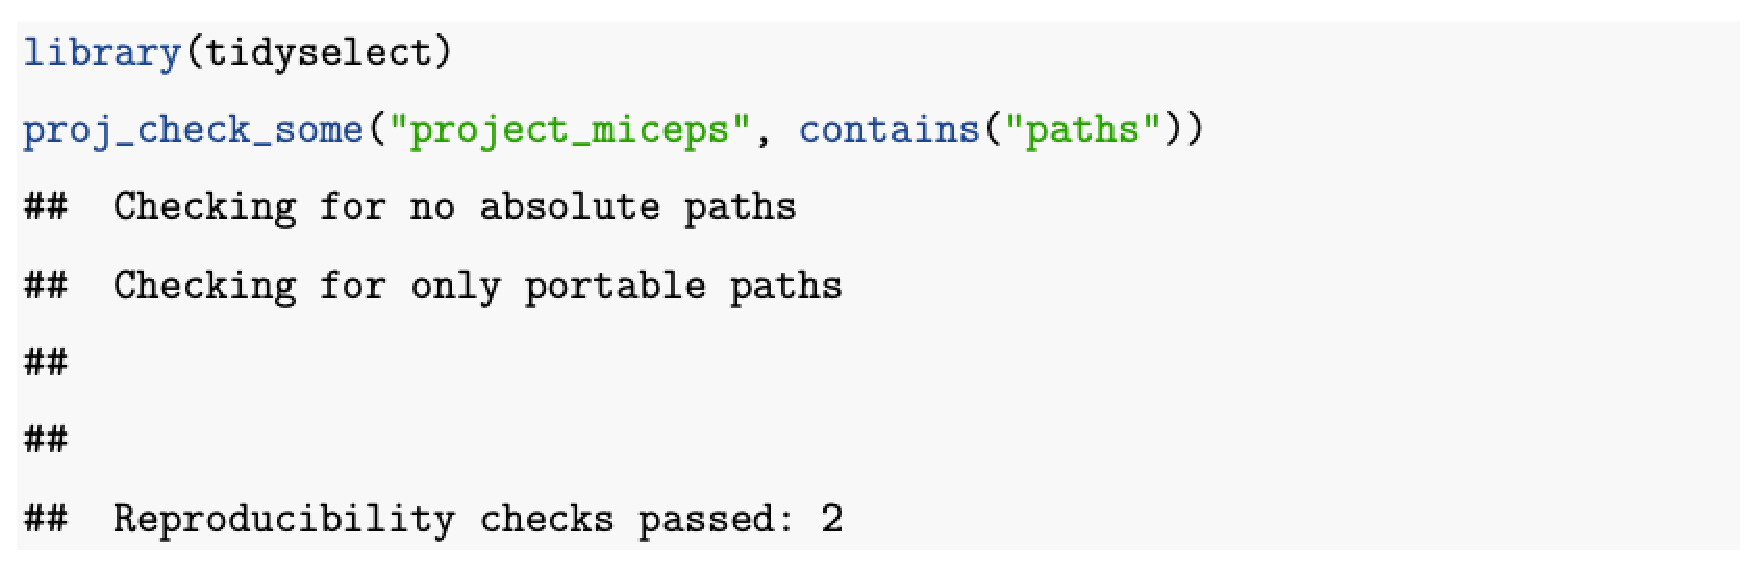
\includegraphics[height=12pc,width=180mm]{fig-5}}

\vskip 0.25in


The \textit{proj\_analyze()} function creates a report documenting the structure of a data analysis project. This report contains information about all packages referenced in code, the files present in the directory and their types, suggestions for moving files to create a more organized structure, and a list of reproducibility-breaking file paths used in code.

\vskip 0.25in

\centerline{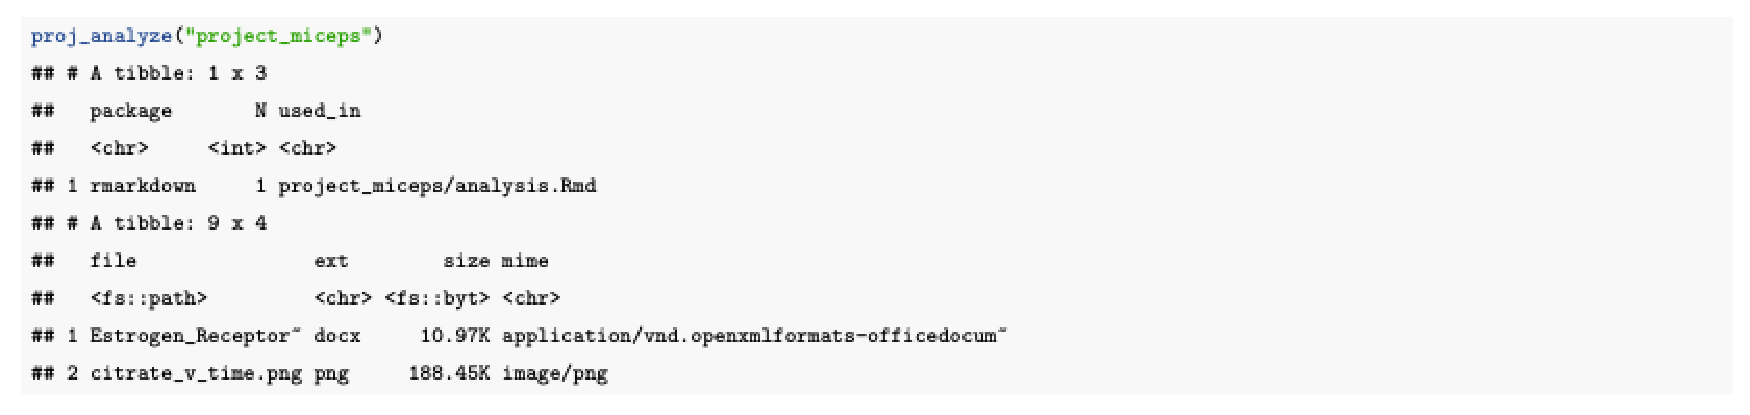
\includegraphics[height=10pc,width=180mm]{fig-6}}
\centerline{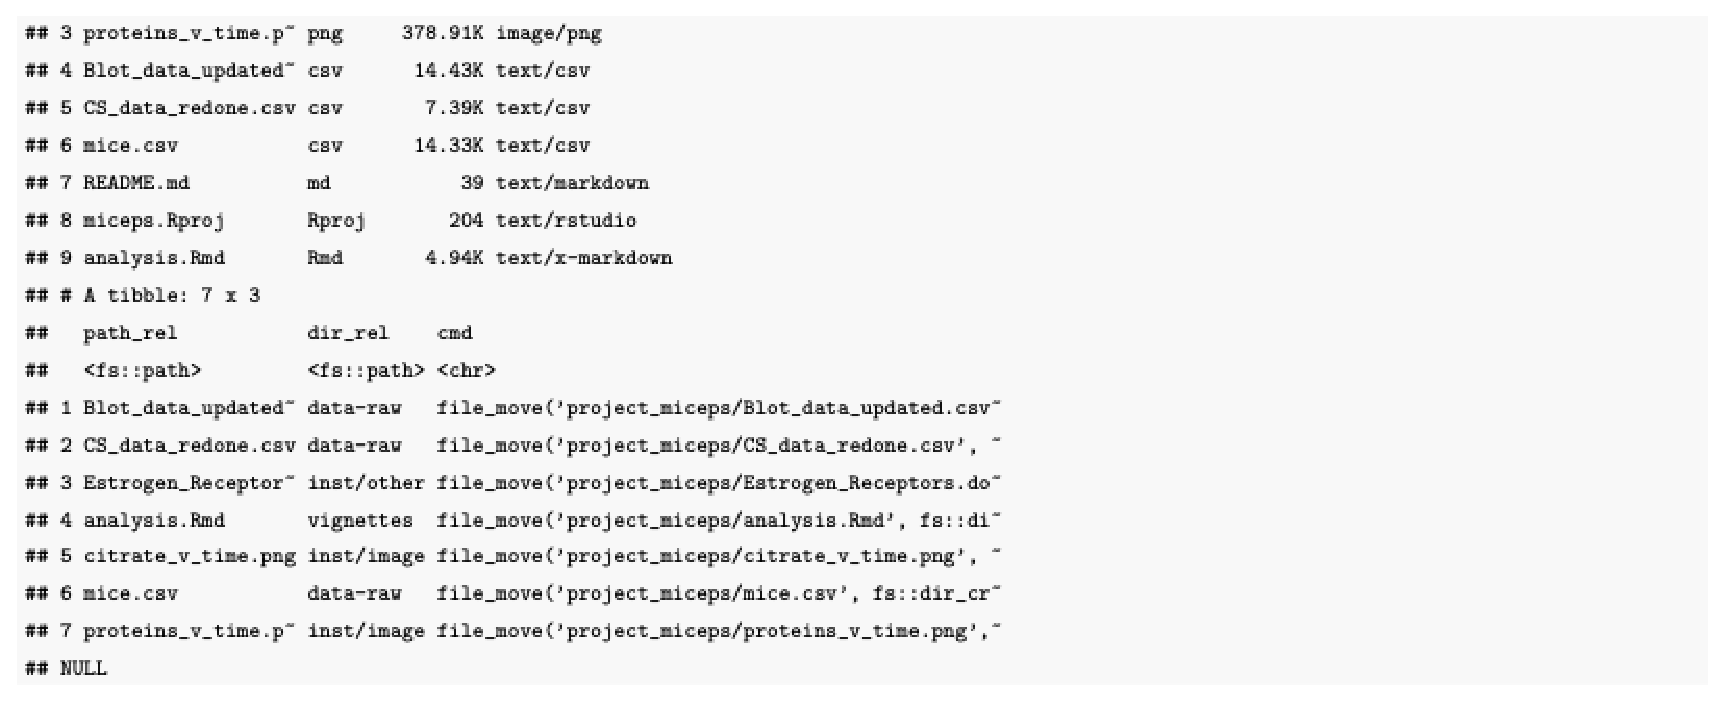
\includegraphics[height=15pc,width=180mm]{fig-7}}

\vskip 0.25in

\textbf{fertile} also contains logging functionality, which records commands run in the console that have the potential to affect reproducibility, enabling users to look at their past history at any time. The package focuses mostly on package loading and file opening, noting which function was used, the path or package it referenced, and the timestamp at which that event happened.
Users can access the log recording their commands at any time via the \textit{log\_report()} function:

\vskip 0.25in

\centerline{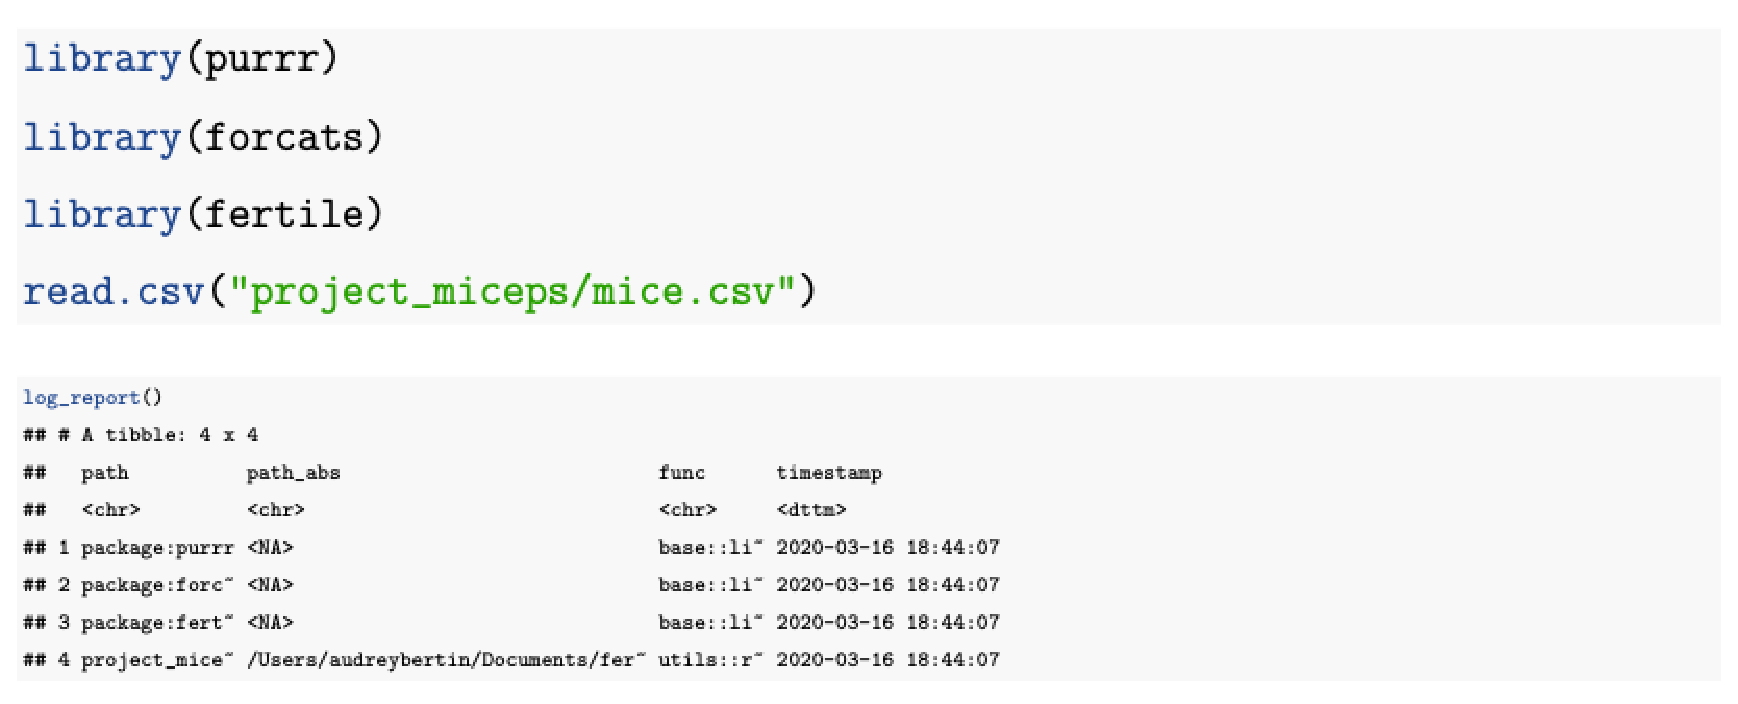
\includegraphics[height=15pc,width=180mm]{fig-8}}

\vskip 0.25in

The log, if not managed, can grow very long over time. For users who do not desire such functionality, \textit{log\_clear()} provides a way to erase the log and start over.

\vskip 0.25in

\centerline{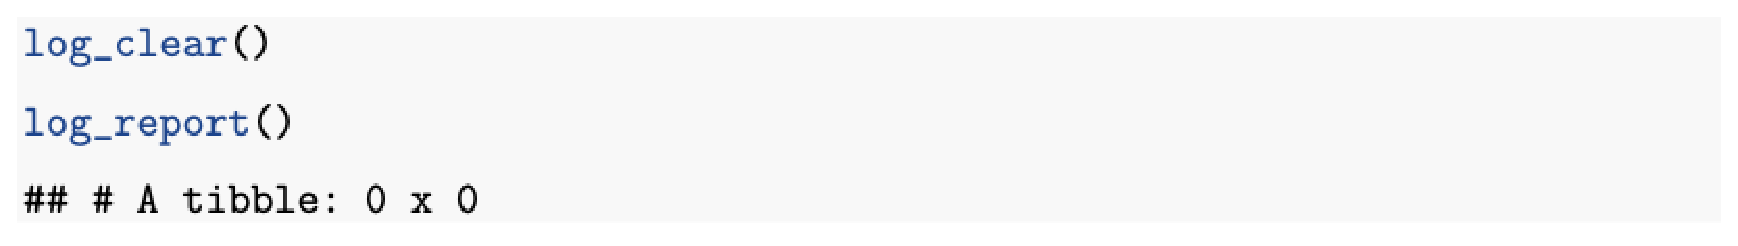
\includegraphics[height=5pc,width=180mm]{fig-9}}

\vskip 0.25in


\subsection{Utility Functions}

\textbf{fertile} also provides several useful utility functions that may assist with the process of data analysis. 


\subsubsection{File Type Checks}

There are several functions that can be used to check the type of a file: 

\vskip 0.25in

\centerline{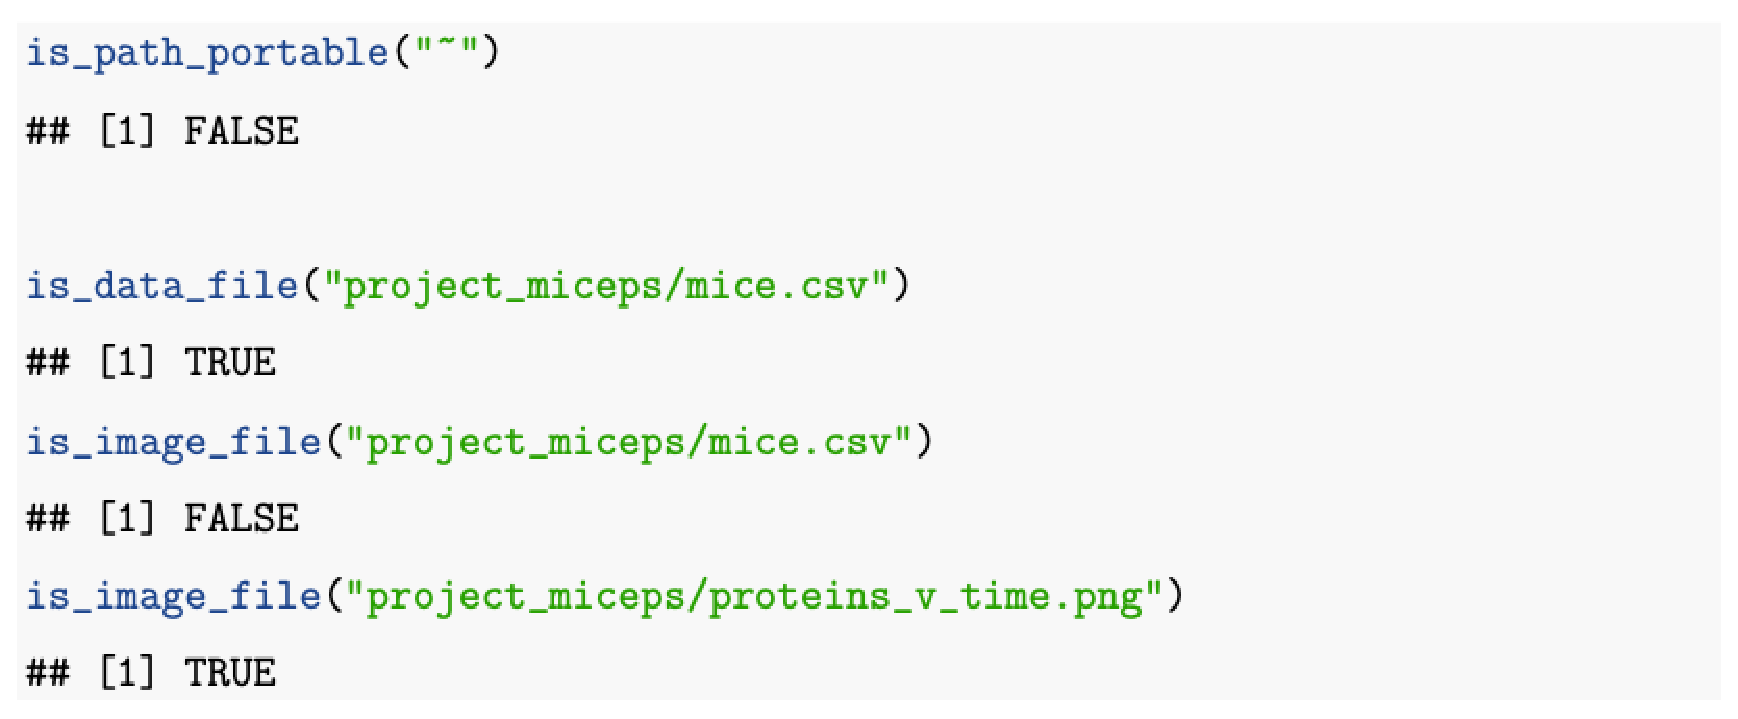
\includegraphics[height=15pc,width=180mm]{fig-10}}

\vskip 0.25in

\subsubsection{Temporary Directories}

The \textit{sandbox()} function allows the user to make a copy of their project in a temporary directory. This can be useful for ensuring that projects run properlt when access to the local file system is removed.

\vskip 0.25in

\centerline{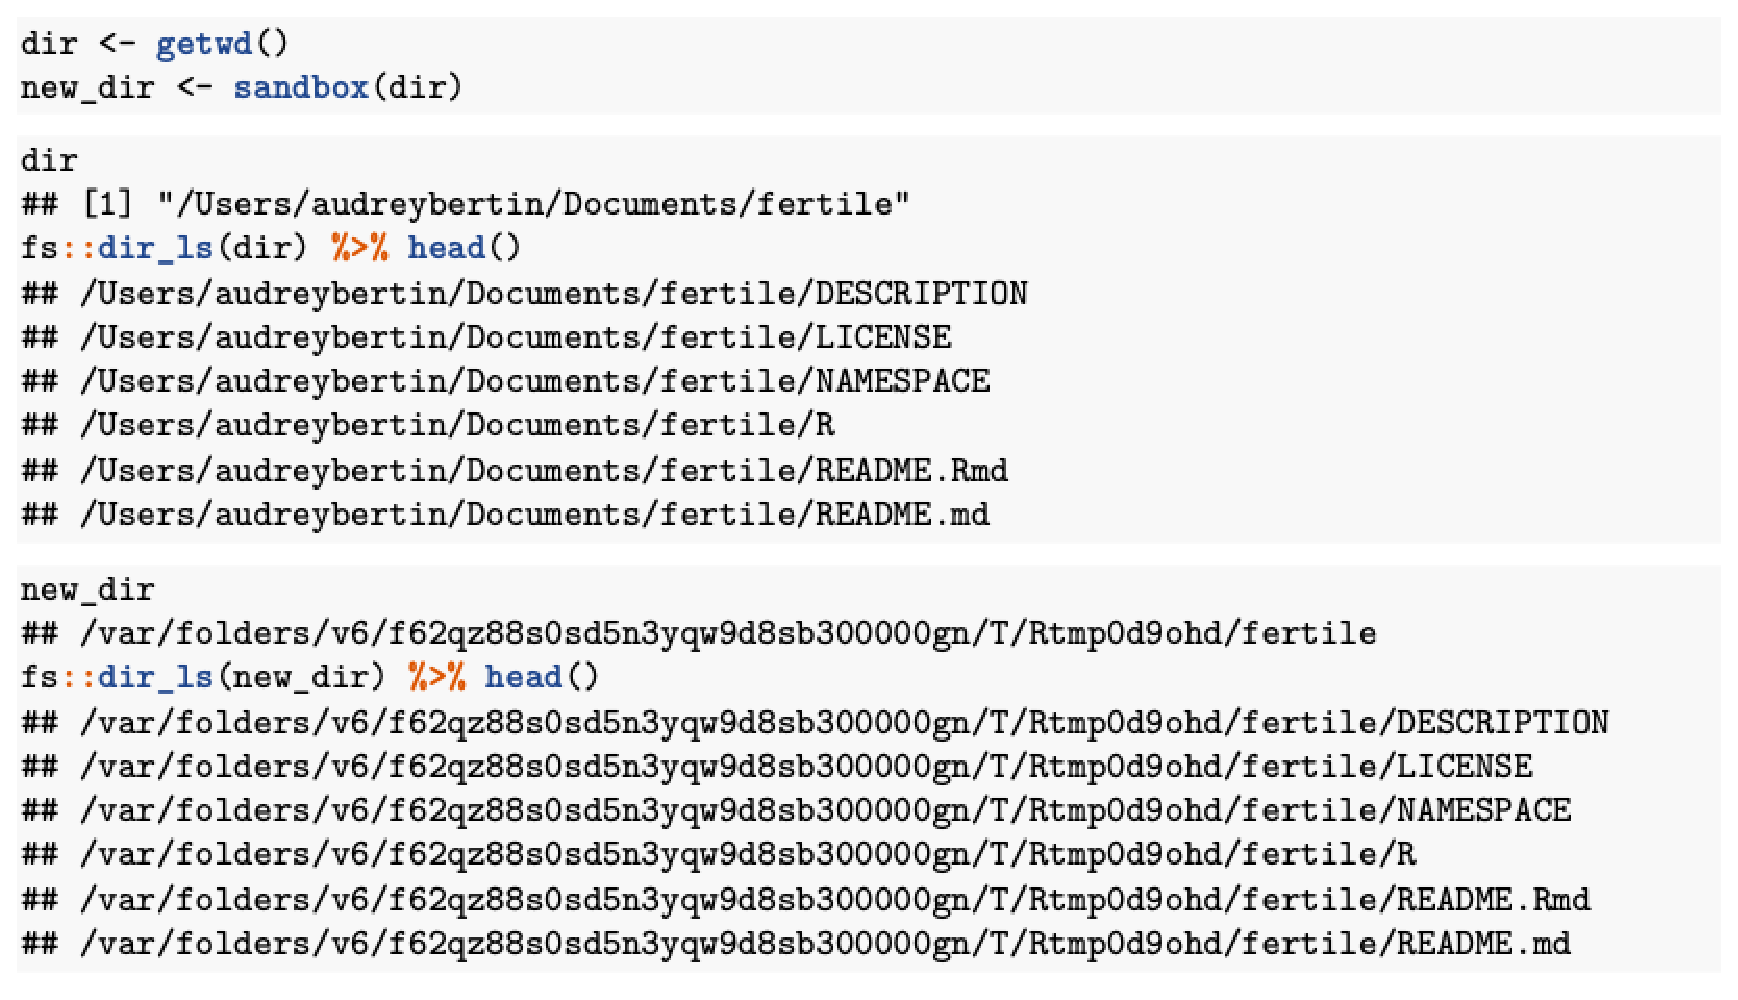
\includegraphics[height=22pc,width=180mm]{fig-11}}

\vskip 0.25in

\subsubsection{Managing Project Dependencies}


One of the challenges with ensuring that work is reproducible is the issue of dependencies. Many data analysis projects reference a variety of R packages in their code. When such projects are shared with other users who may not have the required packages downloaded, it can cause errors that prevent the project from running properly. 

The \textit{proj\_pkg\_script()} function assists with this issue by making it simple and fast to download dependencies. When run on an R project directory, the function creates a \textit{.R} script file that contains the code needed to install all of the packages referenced in the project, differentiating between packages located on CRAN and those located on GitHub.


\vskip 0.25in

\centerline{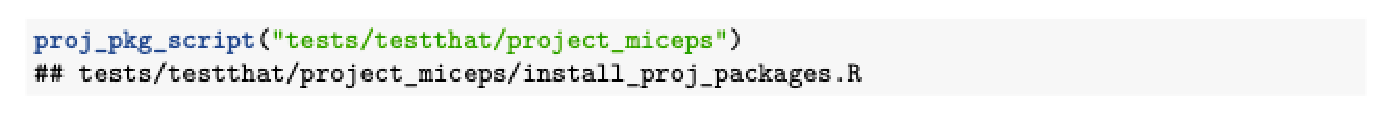
\includegraphics[height=3pc,width=180mm]{fig-12}}

\vskip 0.25in

\centerline{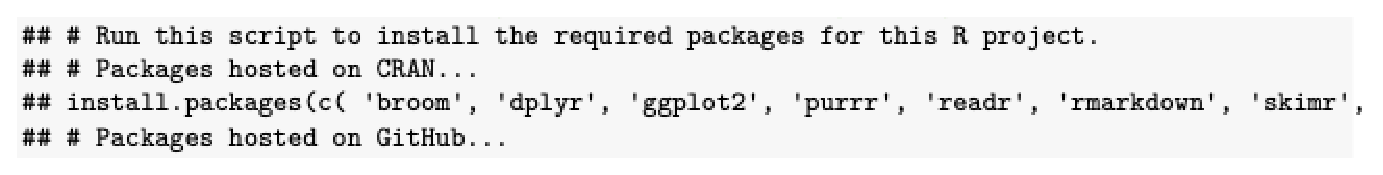
\includegraphics[height=4pc,width=180mm]{fig-13}}

\vskip 0.25in



\subsection{Sample Use Cases}

\vskip 0.25in

\subsubsection{Introductory Data Science Student}

Susan is taking an introductory data science course. This is her first time learning how to code, and she has not yet been exposed to ideas of research reproducibility. Her professor has assigned a data analysis project which must be completed in R Markdown. The project requires her to read in a data file located on her computer and use it to produce a graph.

She reads in the data, makes the graph, and knits her \textit{.Rmd} file. It compiles successfully, so she submits the assignment. The next day, she receives an email from her professor saying that her assignment failed to compile and that she needs to make changes and try again.

Susan doesn't understand why it didn't work on the professor's computer when it did on her own. The professor recommends that she install \textbf{fertile} and run \textit{proj\_check()} on her assignment. She does this and gets a message informing her she used an absolute path to open her dataset, and she should use a relative path. She looks up what this means and then uses the new information to update her assignment. She resubmits and her second attempt is successful.

On future projects, she always loads and runs \textbf{fertile} to make sure her work is okay before submitting.

\subsubsection{Experienced R User}

Emma is a post-doc, with several years of R experience. She is familiar with some basic rules of reproducibility--file paths should always be relative and randomness should always be associated with a seed--but has never needed to pass any sort of reproducibility check before because her professors never emphasized that.

She has just finished a research project and is looking to submit her work to a journal. When researching the journal to which she is interested in submitting, she discovers that it has high standards for research reproducibility and a dedicated editor focusing on that aspect of submission. She goes online and finds the journal's guidelines for reproducibility. They are more complete than any guidelines to which she has previously been required to conform. In addition to notes about file paths and randomness, the journal requires a clean, well-organized folder structure, broken down by file category and stripped of files that do not serve a purpose. In order to be approved, submissions must also have a clear build chain and an informative \textit{README} file.

Unsure of the best way to achieve this structure, Emma goes online to find help. In her search, she comes across \textbf{fertile}. She downloads the package, and in only a handful of commands, she identifies and removes excess files in her directory and automatically organizes her files into a structure reminiscent of an R package. She now meets the guidelines for the journal and can submit her research.


\section{Conclusion}\label{sec4}


\textbf{fertile} is an R package that lowers barriers to reproducible data analysis projects in R, providing a wide array of checks and suggestions addressing many different aspects of project reproducibility, including file organization, file path usage, documentation, and dependencies.

\textbf{fertile} is meant to be educational, providing informative error messages that show how the ways in which the mistakes the user is making are problematic, as well as sharing recommendations on how to fix them. The package is designed in this way so as to promote a greater understanding of reproducibility concepts in its users, with the goal of increasing the overall awareness and understanding of reproducibility in the R community.

The package has very low barriers to entry, making it accessible to users with various levels of background knowledge. Unlike many other R packages focused on reproducibility that are currently available, the features of \textbf{fertile} can be accessed almost effortlessly. Many of the retroactive features can be accessed in only two lines of code requiring minimal arguments, and some of the proactive features can be accessed with no additional effort beyond loading the package. This, in combination with the fact that \textbf{fertile} does not focus on one specific area of reproducibility, instead covering (albeit in less detail) a wide variety of topics, means that \textbf{fertile} makes it easy for data analysts of all skill levels to quickly gain a better understanding of the reproducibility of the work.

In the moment, it often feels easiest to take a shortcut—to use an absolute path or change a working directory. However, when considering the long term path of a project, spending the extra time to improve reproducibility is worthwhile. \textbf{fertile}'s user-friendly features can help data analysts avoid these harmful shortcuts with minimal effort.

\section{Future Work}\label{sec5}

\subsection{Package Features}

The process of ensuring true reproducibility is highly complex and challenging. There are a significant number of components, many of which are described in \hyperref[sec2]{Section 2}, which must all be in place for work to be reproducibile. \textbf{fertile}, in its current version, addresses the vast majority of these in some way. However, there are several areas where further development to extend the available features of the package would be beneficial. These include the following:

\begin{itemize}
  \item Expanding dependency management features to include R session information and package version numbers in addition to package names.
  \item Expanding code and documentation style features to analyze whether code has been properly commented in addition to checking for a \textit{README} and tidy code style.
  \item Adding \textit{make}-like functionality that can analyze an R project structure and files and use this information to generate a Makefile. This Makefile would have information about target files and their prerequisites and would assist with making sure that re-running an analysis is done as quickly as possible by ensuring that only the necessary code and files that have been updated are run when rebuilding and re-running code.
\end{itemize}


\subsection{Testing Effectiveness}

\textbf{fertile} is designed to: 

\begin{itemize}
\item[1] Be simple enough that users with minimal R experience can use the package without issue,
\item[2] Increase the reproducibility of work produced by its users, and
\item[3] Educate its users on why their work is or is not reproducibile and provide guidance on how to address any problems.
\end{itemize}

Anecdotal evidence and user feedback is useful, providing a baseline knowledge of whether these goals are being met. However, in order to truly test whether the package is successful in achieving its design goals, an experiment is necessary.

To test \textbf{fertile}'s effectiveness, we began an initial randomized control trial of the package on an introductory undergraduate data science course at Smith College in Spring 2020, comparing one group of students that received the package functions in their R environment to one that did not. Unfortunately, however, the trial had to be posponed after the COVID-19 pandemic significantly altered the experimental conditions at the midpoint of testing. 

We hope to continue this experimentation and gather data on \textbf{fertile}'s effectiveness once the higher education environment returns to a relatively stable state. 


\nocite{*}% Show all bib entries - both cited and uncited; comment this line to view only cited bib entries;
\bibliography{wileyNJD-APA}%

\section*{Author Biography}

\begin{biography}{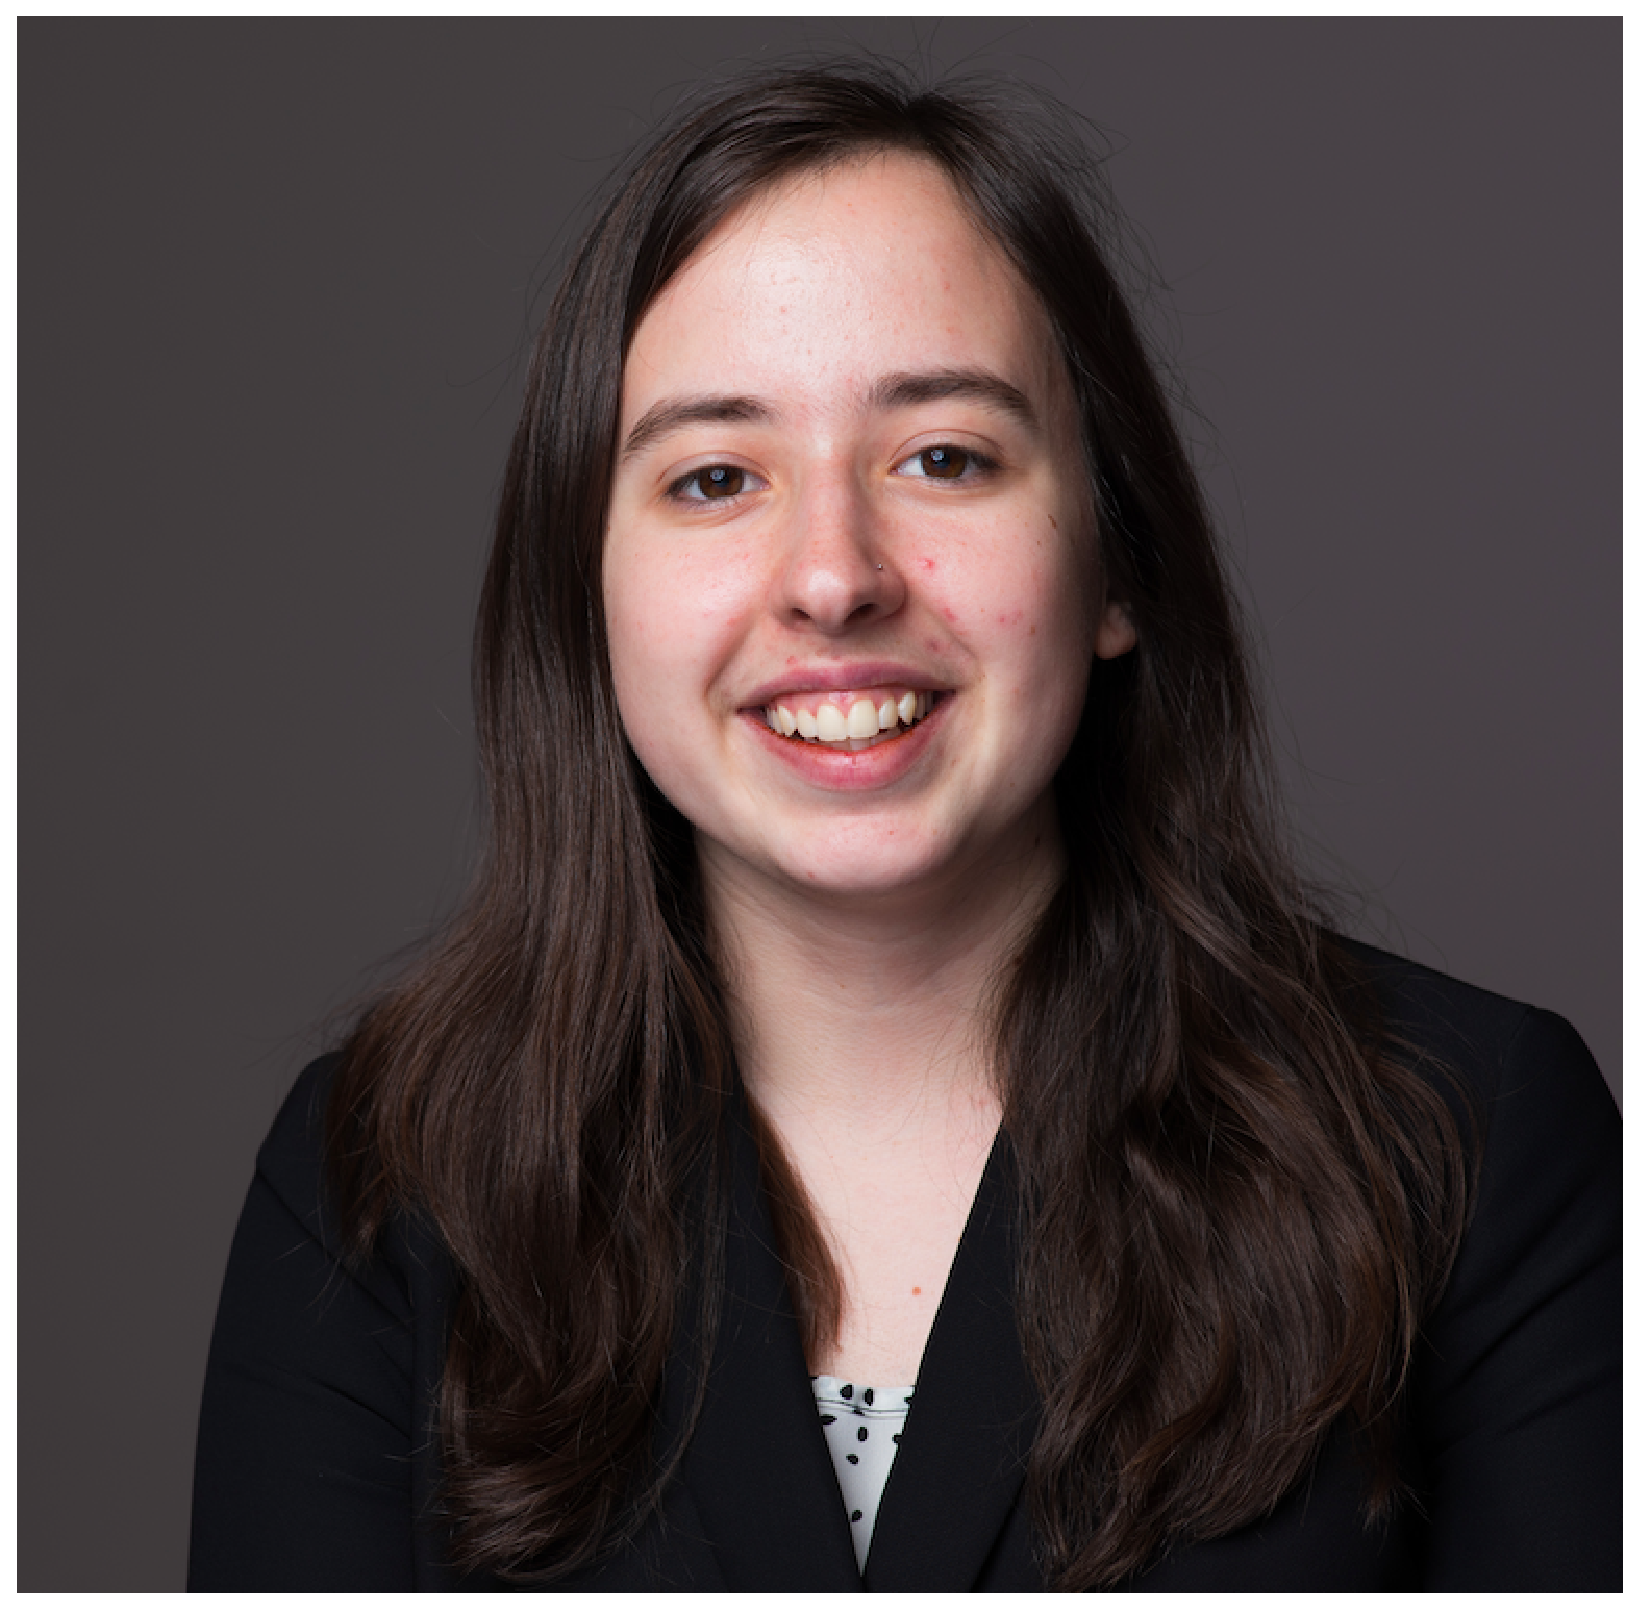
\includegraphics[width=70pt,height=70pt]{audrey_bio}}{\textbf{Audrey Bertin} is an undergraduate student at Smith College intending on completing a Bachelor of arts in Statistical and Data Sciences and Public Policy in Spring 2021. Audrey is a recipient of Smith College's prestigious Zollman Scholarship and has participated in extensive research with faculty throughout her time at the college. Her research interests include data and science communication, data protection and privacy, algorithmic bias and injustice, and using data science for social good.

}
\end{biography}


\begin{biography}{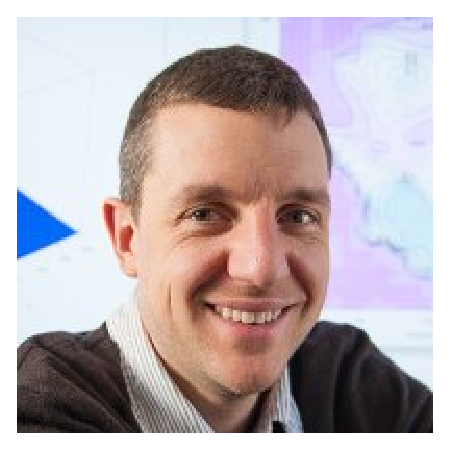
\includegraphics[width=70pt,height=70pt]{ben_bio}}{\textbf{Benjamin S. Baumer} is an associate professor in the Statistical and Data Sciences program at Smith College. Ben is a co-author of The Sabermetric Revolution, Modern Data Science with R, and the second edition of Analyzing Baseball Data with R. Ben has received the Waller Education Award from the ASA Section on Statistics and Data Science Education, the Significant Contributor Award from the ASA Section on Statistics in Sports, and the Contemporary Baseball Analysis Award from the Society for American Baseball Research. His research interests include sports analytics, data science, statistics and data science education, statistical computing, and network science.}
\end{biography}

\end{document}
